\begin{comment}
\begingroup
\begin{figure}[!ht]
  \centering
  \subfigure[]{\includegraphics[width=0.2\linewidth]{}}\label{Chap:Al/Vac:fig:}
  \subfigure[]{\includegraphics[width=0.2\linewidth]{}}\label{Chap:Al/Vac:fig:}
\caption[]{}
  \label{Chap:Al/Vac:fig}
\end{figure}
\endgroup
\end{comment}

Nucleation and growth theories of precipitates in solids are critical to guide the design of structural alloys, because two fundamental principles need to be met: 1) high ductility during processing stages, 2) high strength during the serving stage. However, classical nucleation theories and traditional \ac{KMC} method based on \acf{BEP} relationship fail to provide quantitative guidance for the development of multi-component alloys because of the large number of element types. On the other hand, accurate on-the-fly \ac{KMC} simulations requires costly \ac{NEB} calculations from \ac{DFT}, which is not affordable. In this study, we developed a method combining \ac{KMC} and \ac{NN} functions to study the early transition behavior from supersaturated solid solution to \ac{GP} zone of Al 7000 series alloys. A \ac{NN} function is trained on several thousand accurate \ac{NEB} calculations using \ac{DFT}.

\section{Introduction}
\label{Chap:Al/Vac:section:Intro}

7000 series Al alloys developed for aerospace applications have high specific strength in the peak-aged condition. Carmakers are exploring options for using stamped 7000 series sheets in structural applications in cars and trucks, from both the manufacturing perspective and the performance perspective. Their widespread implementation in the automotive industry for body and closure applications can achieve vehicle lightweighting goals if the challenges of the component forming and fabrication can be overcome. \cite{fridlyander2002aluminum,hirsch2011aluminium,hirsch2014recent}

\begingroup
\begin{figure}[!ht]
  \centering
  \subfigure{\includegraphics[width=1.0\linewidth]{Chap5/plots/Picture1.png}}
\caption[Schematics of fabrication process of 7000 series Al sheet alloy parts in automobile industry.]{Schematics of fabrication process of 7000 series Al sheet alloy parts in automobile industry. The corresponding changes of illustrated atomistic structures of precipitates during this process are also plotted (blue: Al atoms, other colors: solutes).}
  \label{Chap:Al/Vac:fig1}
\end{figure}
\endgroup

As show in Fig. \ref{Chap:Al/Vac:fig1}, conventional automotive mechanical forming processes such as stamping and hemming, involve room temperature forming of Al sheet alloys in the as-quenched state when alloys have high ductility and formability, followed by artificial aging during the paint bake operation. Due to fast (often within 30 minutes after quenching) and continuously varying natural aging characteristics of current 7000 series alloys, the formability decreases very rapidly and keeps changing as the aging time increases, necessitating costly steps such as warm stamping and coupled solutioning-quenching-stamping operations in a narrow time window. \cite{bryant1999effects,li2004biaxial} These variations of formability and other mechanical properties are all related to the evolution of atomistic structures of precipitates during the sheet processing procedures.

As a result, to understand and to control the nucleation and early stages of precipitation kinetics will have a great impact in automotive applications of age-hardened, light-weight alloys. \cite{deschamps1998influence,banhart2011kinetics,liang2012kinetics,deschamps2014precipitation} The nucleation and growth of precipitates in Al-Zn-Mg-based alloys is currently understood to follow the following sequence: supersaturated solid solution (SSSS) $\rightarrow$ \acf{VRC} $\rightarrow$ \acf{GP} zones (nanoscale coherent Mg/Zn-rich clusters) $\rightarrow$ $\eta'$ (semi-coherent Mg-Zn-Al precipitates with high Zn/Mg ratio) $\rightarrow$ $\eta$ (incoherent $\text{MgZn}_\text{2}$). \cite{ragueneau2000review,deschamps2014precipitation,berg2001gp,chung2018transmission} During natural aging, the majority of precipitates are \ac{VRC} and \ac{GP} zones, even though $\eta'$ can also be found in some cases. \cite{mukhopadhyay1994guinier} Therefore, in this chapter, how to retard the nucleation and growth of \ac{VRC} and \ac{GP} zones in 7000 series Al alloys during natural aging without reversely effects on the precipitation kinetics during subsequent artificial aging will be focused on.


As we previously mentioned in Section. \ref{Chap:Mech:NN}, due to the simplicity of analytical formulas and costly \ac{DFT} calculations, empirical potentials can only focus on a limited number of material properties of the fitted system. As the number of species included in the system increases, it is also getting more difficult to fit the desired empirical potential. For simple vacancy-bulk diffusion or surface diffusion events, \acf{BEP} relationship, based on bond counting model up to a certain cutoff, were commonly used. \cite{soisson1996monte, soisson2010atomistic} However, this method oversimplified the contribution of atomistic local environments and elastic energetics. In this chapter, we will use a machine learning method to predict accurate diffusion barriers for multi-component systems.

\newpage
\begingroup
\begin{figure}[!ht]
  \centering
  \subfigure{\includegraphics[width=0.8\linewidth]{Chap5/plots/E-EB.pdf}}
\caption[Correlation between diffusion barriers and energy differences for multi-component Al-Mg-Zn systems]{Correlation between diffusion barriers and energy differences for multi-component Al-Mg-Zn systems.}
  \label{Chap:Al/Vac:fig2}
\end{figure}
\endgroup


Based on the above hypotheses, the proposed work will be organized as the following tasks. We will apply first-principles calculations to obtain a training set for diffusion barriers of a single vacancy in various local environments. Then, we will construct machine-learning interatomic potentials for multi-component Al-Zn-Mg systems without/with suggested trace solute elements. These potentials will be used in \ac{KMC} simulations and molecular static/dynamic(MS/MD) simulations to predict the structures/compositions of \ac{VRC}/\ac{GP} zones and their effects on hardness increments during natural aging with the help of phenomenological strengthening models.
\section{Fitting Vacancy Migration Barriers using Neural Network}
\label{Chap:Al/Vac:section:NN}

The calculations that provided the energetics used to evaluate energy differences and activation barriers before and after vacancy jump in Al-Mg-Zn alloys were implemented by \ac{DFT} together with \acf{CI-NEB} in the \ac{VASP} software with VTST package from Henkelman's group\cite{henkelman2000climbing,henkelman2000improved}. The \acf{NEB} is a general method for finding saddle points and minimum energy paths between the atomic configurations of the known initial and final states. This method works by optimizing a certain number of intermediate images along the reaction path. Each image finds the lowest possible energy while maintaining linear spline spacing to neighboring images. This is done by adding artificial spring forces along with the band between images and by projecting out the force component parallel to the band due to the interatomic potential. The \ac{CI-NEB} method modifies the \ac{NEB} method in a way that the highest-energy image is pushed up to the saddle point by trying to maximize its energy along with the band and minimize in all other directions. When the algorithm converges, the highest-energy image is at the exact saddle point, so a smaller number of intermediate images is needed in \ac{CI-NEB} than \ac{NEB}. With this setup, we can use high-throughput calculations to extract forward/backward activation barriers by calculating the energy differences between the image of the highest energy and the initial/final image.

\begingroup
\begin{figure}[!ht]
  \centering
  \subfigure[]{\includegraphics[width=0.65\linewidth]{Chap5/plots/kpoints_converge.pdf}}
  \subfigure[]{\includegraphics[width=0.65\linewidth]{Chap5/plots/kpoints_speed.pdf}}
\caption[Plot of k-point grids convergence and efficiency test on vacancy migration barrier.]{Plot of k-point grids convergence and efficiency test on vacancy migration barrier. (a) Vacancy migration barriers along reaction coordinates of (1$\times$1$\times$1), (2$\times$2$\times$2), and (4$\times$4$\times$4) k-point grid setups are tested. (b) The total time elapsed using (1$\times$1$\times$1), (2$\times$2$\times$2), and (4$\times$4$\times$4) k-point grid setups are plotted. A 256-atom randomly generated Al-Mg-Zn configuration is used for this test.}
\label{Chap:Al/Vac:fig:kpoints}
\end{figure}
\endgroup

Pseudopotentials based on the \ac{PAW} method were employed for the elemental constituents with the \ac{GGA} of \ac{PBE} for the exchange-correlation energy functional, $\mu_{xc}$, with the interpolation formula of Vosko et al. \cite{vosko1980accurate}. Using plane-wave cutoff energy of 450.0 eV, the total energy for all models of initial and final images was converged to $10^{−7}$ eV/cell. The reciprocal space of bulk supercells was sampled with (2$\times$2$\times$2) k-point grids. Each grid was generated using the Monkhorst-Pack scheme \cite{monkhorst1976special}. In Figure \ref{Chap:Al/Vac:fig:kpoints}, we plotted the vacancy migration barrier of a 256-atom randomly generated Al-Mg-Zn configuration using different k-point grids. In subplot (a), (2$\times$2$\times$2) and (4$\times$4$\times$4) k-point grids do not have a significant difference on reaction coordinates and migration barrier. However, running on a 120-core machine, (4$\times$4$\times$4) k-point takes 5 times longer simulation time. Considering the efficiency, we choose (2$\times$2$\times$2) k-points with almost no accuracy compromise. A (4$\times$4$\times$4) conventional fcc supercell with a single vacancy embedded was used for these calculations. For activation barrier calculations, 5 images between relaxed initial and final images were used. A spring constant was set to 5 $\text{eV}/\angstrom^2$. The force convergence criteria for all models was set to be less than 0.05 $\text{eV}/\angstrom$. The force-based quick-min optimizer was used to make \ac{NEB} calculations stable for high local concentration cases\cite{sheppard2008optimization}.


We calculated lattice constant for Al-Mg-Zn alloys based on the chemical composition of  7075 Al alloy. A (4$\times$4$\times$4) conventional supercell with 256 atoms was used to generate random lattice occupations by solute atoms using \acfp{SQS} method \cite{zunger1990special}. The types of 256 atoms were chosen to be 244 Al atoms, 7 Mg atoms, and 5 Zn atoms, which is within the concentration range of Al 7075 alloy. The obtained lattice constant is 4.05838 \angstrom, which is roughly equal to the lattice constant of pure Al (4.041\angstrom from the same DFT setup parameters) considering that Zn and Mg atomic weights are not high\cite{haas2009calculation}.


Our \ac{NN} model training set contains mainly from the calculated vacancy migration barriers in two different types of supercells, as shown in Figure \ref{Chap:Al/Vac:fig:atomic_illu}: 1) (4$\times$4$\times$4) randomly generated solid-solution structures with different local concentrations around the jump pair, which is defined by the two lattice sites for the vacancy before and after the migration event. 2) (2$\times$2$\times$2) ordered structures embedded in (4$\times$4$\times$4) pure Al. The first training set is good for simulating vacancy migration of a very early stage, during which Al alloy is still in the solid-solution state. The second training set is designed to accurately describe the behavior of vacancy migrations across/along the boundary between solid-solution Al and ordered clusters/precipitates, and moving inside the ordered phases. The atomic structures of ordered phases are randomly chosen from the proposed GP zone structures from \cite{berg2001gp} and low energy ordered $\text{L1}_\text{0}, \text{L1}_\text{2}, \text{L1}_\text{0}^*, \text{W2}, \text{CH}, \text{L1}_\text{2}^*, \text{Z1}$ structures of Au-Fe from \cite{zhuravlev2017phase} with random perturbations in lattice occupations. The atomic structures were generated using our in-house code KNN2\cite{Zhang2020KNN2}. 

\begingroup
\begin{figure}[!ht]
  \centering
  \subfigure[]{\includegraphics[width=0.49\linewidth]{Chap5/plots/ss_atomic.jpg}}
  \subfigure[]{\includegraphics[width=0.49\linewidth]{Chap5/plots/ordered_atomic.jpg}}
\caption[Atomistic pictures of (4$\times$4$\times$4) supercells containing 256 atoms.]{Atomistic pictures of (4$\times$4$\times$4) supercells containing 256 atoms. (a) One typical (4$\times$4$\times$4) randomly generated solid-solution structure. (b) One typical (2$\times$2$\times$2) randomly chosen ordered structures embedded in (4$\times$4$\times$4) pure Al. Light green, dark green, and red atoms are Al, Mg, and Zn, respectively. The small gray atom represents the location of vacancy.}
\label{Chap:Al/Vac:fig:atomic_illu}
\end{figure}
\endgroup


Many different machine learning/deep learning models are widely used to study materials science problems\cite{bartok2010gaussian,behler2011atom,szlachta2014accuracy,artrith2016implementation,mehta2014exact,artrith2017efficient}. For our particular case, the feed-forward Artificial Neural Network (ANN) is chosen, as it provides a general frame to map non-linear input (atomic species of neighboring environment) to a continuous regressand (vacancy migration barrier). It is well known that a sufficiently large number of hidden neurons can approximate any continuous multivariate function\cite{hornik1989multilayer}. This property gives us the most expandability of this framework when the system needs to go even further complicated in terms of the number of species considered. 

\begin{table}[!htbp]
\centering
\caption[Atom species encoding map for the \acf{NN} input layer.]{Atom species encoding map for the \acf{NN} input layer. Here, ``Vac'' represents vacancies.}
\label{Chap:Al/Vac:tab:mapping}
\begin{tabular}{cc}
\\
\hline
\hline
Species & Encoding  \\ \hline
Al & 1.0 \\
Mg & 2.0 \\
Zn & 3.0 \\
Vac & 4.0 \\
\hline
\hline
\end{tabular}
\end{table}

\begingroup
\begin{figure}[!ht]
  \centering
  \subfigure{\includegraphics[width=0.5\linewidth]{Chap5/plots/2nn.png}}
\caption[Illustration of atomic structures of the $\text{1}^{st}$ and $\text{2}^{nd}$ nearest neighbors surrounding the jumping pairs.]{Illustration of atomic structures of the $\text{1}^{st}$ and $\text{2}^{nd}$ nearest neighbors surrounding the jumping pairs (the lattice sites of the vacancy before and after a migration event). The 26 neighboring atoms have 2-fold symmetry, mirror symmetry along Y-Z plane, and mirror symmetry along the X-Y plane.}
\label{Chap:Al/Vac:fig:2nn}
\end{figure}
\endgroup

The output layer of our \ac{NN} model predicts vacancy migration barriers in a 1-D continuous space. Like the Ising model, the input layer was chosen to be 27 discrete numbers representing atom species that occupy all the $\text{1}^{st}$ and $\text{2}^{nd}$-nearest-neighbor lattice sites of the vacancy before and after the migration events (the jump pair), as shown in Table \ref{Chap:Al/Vac:tab:mapping}. Among the 27 numbers, the first one indicates the type of atom that will be swapped with the vacancy. The rest 26 numbers represent the neighboring atoms of the jump pair up to their $\text{2}^{nd}$ nearest neighbors (each lattice site of the jump pair has 12  $\text{1}^{st}$ nearest neighbors and 6 $\text{2}^{nd}$ nearest neighbors. In addition, both of them share 10 neighbors in common. So 26 = (12 + 6)$\times$2-10). All these 26 atoms as shown in Figure \ref{Chap:Al/Vac:fig:2nn}, where the X, Y, and Z axes are defined as the following. In principle, X, Y, and Z directions can be any orthogonal vectors, as long as they are consistent during the training and serving stages of the simulation. Here, we choose Y as a $\langle$110$\rangle$ vector along the vacancy jumping direction; X is along another $\langle$1$\bar{1}$0$\rangle$ vector perpendicular to Y; Z is along the $\langle$001$\rangle$ vector perpendicular to both X and Y axes. Beside the first number for the swapped site for the vacancy jump, all the left 26 numbers are arranged in their geographical order, so their position will always respond to the same input neuron in the \ac{NN} architecture. In addition, this cluster of 26 neighboring atoms also has 2-fold symmetry  ($R_{2 fold} = \begin{bmatrix} 1 & -1 & 0 \\-1 & -1 & 0 \\0 & 0 & -1 \\\end{bmatrix}$), mirror symmetry along Y-Z plane ($R_{x mirror} = \begin{bmatrix} -1 & 1 & 0 \\1 & 1 & 0 \\0 & 0 & 1 \\\end{bmatrix}$), and mirror symmetry along the X-Y plane($R_{z mirror} = \begin{bmatrix} 1 & -1 & 0 \\1 & 1 & 0 \\0 & 0 & -1 \\\end{bmatrix}$). Therefore, for one jumping event, the vacancy migration barrier is taken as the average of the four symmetric configurations of the 26 neighboring atoms to have a rotation-invariant prediction. Details of this method is described in Algorithm \ref{algo:encode}. By using several layers of hidden neurons between 27 input and the final output, the contribution of pair-wise and triple-wise interactions can be learned.

\begin{figure}[!htb]
  \centering
  \begin{minipage}{.7\linewidth}
    \begin{algorithm}[H]
      \caption{Jumping Pair Encoding Algorithm}\label{algo:encode}
      \begin{algorithmic}[1]
        \State set a reference matrix as a 3$\times$3 identity matrix, $m_0$ = $$\begin{bmatrix} 1 & -1 & 0 \\1 & 1 & 0 \\0 & 0 & 1 \\\end{bmatrix}\quad$$.
        
        \State determine the jumping direction $v_0 = r_{atom} - r_{vac}$, where $r$ is the coordinates of atom/vacancy. Noting that in the practice, atoms may need to be wrapped according to periodic boundary conditions.
        \State determine all the 26 neighboring atoms of the ghost atom at the vacancy site and the jumping atom within the $2^{nd}$ nearest neighbor distance cutoff.
        \State randomly pick one $2^{nd}$ nearest neighbor atom with coordinates $r_1$ of the vacancy atom, and calculate $v_1 = r_{1} - r_{vac}$.
        \State calculate $v_2 = v_0 \cdot v_1$.
        \State concatenate matrix $m_1$ = $\begin{bmatrix} v_0 \\v_1 \\v_2 \\\end{bmatrix}$.
        
        \State calculate rotation matrix $R$ for projecting $m_1$ to the reference coordinate $m_0$. 
        \State rotate coordinates of all the 26 atoms by applying the rotation matrix $R$ to project all the atoms need to encode along the same reference directions. The new coordinates denotes as $r'$. 
        \State encode atoms based on the preset mapping of type, and ascending order in X, Y, and Z coordinates accordingly.
        \State apply for the three rotational matrices, 
        $R_{2 fold} = \begin{bmatrix} 1 & -1 & 0 \\
                                      -1 & -1 & 0 \\
                                      0 & 0 & -1 \\
        \end{bmatrix}\quad$
        $R_{x mirror} = \begin{bmatrix} -1 & 1 & 0 \\
                                         1 & 1 & 0 \\
                                         0 & 0 & 1 \\
        \end{bmatrix}\quad$
        $R_{z mirror} = \begin{bmatrix} 1 & -1 & 0 \\
                                        1 & 1 & 0 \\
                                        0 & 0 & -1 \\
        \end{bmatrix}\quad$
        , to the coordinates $r'$ and encode them use the same method mentioned above.
        
      \end{algorithmic}
    \end{algorithm}
  \end{minipage}
\end{figure}



We implemented the \ac{NN} model using Google's TensorFlow \cite{abadi2016tensorflow} with Keras \cite{chollet2015keras}. TensorFlow is an open-source numerical computation framework using data flow graphs with the ability to derive gradients automatically. Keras is a high-level neural networks API, written in Python and capable of running on top of TensorFlow. The optimized neural network structures were tuned by Talos \cite{Autonomio2019Talos}. The Adam optimizer \cite{kingma2014adam} was used for optimizing weights in the neural network. Xavier uniform initializer \cite{glorot2010understanding} was used to generate the random weights and biases so as to break the symmetry of weighting parameters. The activation functions were chosen to be \acf{ReLu} for all the hidden layers. The activation function for the output layer is chosen to be linear to predict vacancy migration barriers on a continuous scale. Normalization method has also been tested but is not helpful in improving accuracy, as vacancy migration barriers follow a very good normal distribution.  The optimized \ac{NN} architecture can be found in Table \ref{Chap:Al/Vac:tab:NN}. Large neural nets trained on relatively small datasets can overfit the training data. So the dropout as a regularization method is applied to prevent overfitting. This introduces a new hyperparameter, the dropout probability, as listed in Table \ref{Chap:Al/Vac:tab:NN}. Though more complicated \acf{RBM} and many other generative stochastic artificial neural networks can be used as a function approximator, their complexity slows down the \ac{kMC} iterations significantly, so that they are not used here.

\begin{table}[!htbp]
\centering
\caption[Neural network architecture with activation functions and dropout probability of each layer.]{Neural network architecture with activation functions and dropout probability of each layer.}
\label{Chap:Al/Vac:tab:NN}
\begin{tabular}{cccc}
\\
\hline
\hline
Layer & Shape  & Activation  & Dropout Probability\\ 
\hline
Dense & 256    & ReLu       & 0.1                 \\
Dense & 256    & ReLu       & 0.2                 \\
Dense & 128    & ReLu       & 0.0                 \\
Dense & 64     & ReLu       & 0.05                \\
Dense & 64     & ReLu       & 0.0                 \\
Dense & 16     & ReLu       & 0.0                 \\
Dense & 1      & Linear     & N.A.                \\ 
\hline
\hline
\end{tabular}
\end{table}


\begingroup
\begin{figure}[!ht]
  \centering
  \subfigure[]{\includegraphics[width=0.49\linewidth]{Chap5/plots/total.png}}
  \subfigure[]{\includegraphics[width=0.49\linewidth]{Chap5/plots/fit_ordered.png}}
\caption[Predictions accuracy of vacancy migration barriers from neural network surrogate model, compared with DFT calculated results.]{Predictions accuracy of vacancy migration barriers from neural network surrogate model, compared with DFT calculated results. During model training, Equation \ref{Chap:Al/Vac:eq:MSE} was used as the loss function. The orange solid line indicates perfect fitting. Each blue solid dot represents one data point. (a) predictions of all the barriers from DFT training data set. (b) predictions of the barriers in certain ternary ordered structures as the testing data set.}
\label{Chap:Al/Vac:fig:fitting_all}
\end{figure}
\endgroup

\begingroup
\begin{figure}[!ht]
  \centering
  \subfigure[]{\includegraphics[width=0.49\linewidth]{Chap5/plots/total_weighted.png}}
  \subfigure[]{\includegraphics[width=0.49\linewidth]{Chap5/plots/fit_ordered_weighted.png}}
\caption[Predictions accuracy of vacancy migration barriers from neural network model using custom loss function, compared with DFT calculated results.]{Predictions accuracy of vacancy migration barriers from neural network model using custom loss function, compared with DFT calculated results. During model training, Equation \ref{Chap:Al/Vac:eq:custLoss} was used to weigh more on low-energy barriers. The orange solid line indicates perfect fitting. Each blue solid dot represents one data point. The black dashed lines illustrate the confinement introduced by custom loss function with emphasis on low-energy-barrier data points. (a) predictions of all the barriers from DFT training data set. (b) predictions of the barriers in certain ternary ordered structures as the testing data set.}
\label{Chap:Al/Vac:fig:fitting_all_weighted}
\end{figure}
\endgroup

To train the \ac{NN}, two different loss functions are used. The former one is the common \acf{MSE} via:
\begin{equation}
MSE = \frac{1}{N}\sum_{i=1}^{N}({E_a}_{i}^{DFT} - {E_a}_{i}^{NN})^2
\label{Chap:Al/Vac:eq:MSE}
\end{equation}
where $N$ is the number of input data, which can be trained in batch or mini-batch, ${E_a}_i^{DFT}$ is the vacancy migration barrier of $i^{\text{th}}$ data from \ac{DFT} calculation, and ${E_a}_{i}^{NN}$ is from \ac{NN} prediction. As shown in Figure \ref{Chap:Al/Vac:fig:fitting_all}, the model reached a \ac{RMSE} of 0.04313 eV/atom for all the data points. The latter one is a customized loss function as:
\begin{equation}
Loss = \frac{1}{N}\sum_{i=1}^{N}{(1.0 + \alpha (1.5 - {E_a}_{i}^{DFT})({E_a}_{i}^{DFT} - {E_a}_{i}^{NN})^2)}
\label{Chap:Al/Vac:eq:custLoss}
\end{equation}
where $\alpha$ is a tunable knob. A larger $\alpha$ value will weigh more on vacancy migration barriers that are small. In this way, we are able to fit low-energy barriers more accurately, as they are the critical rate-determining steps in a \ac{kMC} simulation. Using this custom loss function, the model reached a \ac{RMSE} of 0.03785 eV/atom for all the data points. Noting that the model trained using the latter loss function is slightly more accurate than the former method because more data points are located far away from 1.5 eV. As we expected, low-energy barriers are predicted with higher accuracy, which can be seen from Figure \ref{Chap:Al/Vac:fig:fitting_all_weighted}.
\newpage
\section{Kinetic Monte Carlo Setup}
\label{Chap:Al/Vac:section:KMC}

Most parts of the \ac{KMC} algorithm were implemented following the approach we discussed in Algorithm. \ref{algo:kMC} of Chap. \ref{chap:meth:KMC}. In this implementation, several points are worth noticing: 1) Event list is determined on the fly. We consider the first nearest neighbor exchange of vacancies. This yields a total of 12 times the total number of vacancies possible events. 2) Then, a \ac{NN} potential is used, instead of traditional empirical potentials or analytical equations, to evaluate diffusion barriers. Noting that all the four symmetry equivalent structures are taken into consideration. 3) At each step, both the forward and backward diffusion barriers of executing the current jump will be calculated to obtain the energy change of the current system, via:
\begin{align}
\Delta E = {E_a}^{forward} - {E_a}^{backward}
\label{Chap:Al/Vac:eq:barrier-EDiff}
\end{align}
where $\Delta E$ is the energy difference between initial and final state, ${E_a}^{forward}$ and ${E_a}^{backward}$, are the forward/backward diffusion barrier, respectively. And the overall energy change as time-evolving is cumulated. 4) In order to boost the system out of low-energy barrier trapping states, a local super-basin method is also implemented based on Ref. \cite{fichthorn2013local}.

For the \ac{KMC} simulations, (30x30x30) supercell containing 108,000 atoms were used. 3240 Mg atoms, 1700 Zn atoms and 1 vacancy atom were randomly chosen among 108,000 atoms. This setup corresponds to $\sim$ 3 atom. \% of Mg, $\sim$ 2 atom. \% of Zn and a vacancy concentration of $\sim$ 1e-6. The probability, $p_k$, of selecting an event $k$ is calculated, via:
\begin{subequations}
\begin{align}
& p_i = r_i / R    \label{Chap:Al/Vac:eq:prob} \\
& r_i = \mu_a * exp(- E_a / k_B T)  \label{Chap:Al/Vac:eq:rate} \\
& R = \sum_{j=1}^N r_j \label{Chap:Al/Vac:eq:R} \\
& \sum_{k=1}^{i-1} p_k < rand < \sum_{k=1}^{i} p_k \label{Chap:Al/Vac:eq:choice}
\end{align}
\end{subequations}
where $\mu_a$ is the diffusion pre-exponential factor, $E_a$ is the diffusion barrier, $k_B$ is the Boltzmann constant, T is the temperature, $N$ is the total number of events, and $rand$ is a random number $\in [0, 1)$. In reality, the diffusion pre-exponential factor, AKA the attempt frequency, and the diffusion barrier depend on the specific configuration \cite{osti_323431,van2001first,le2002kinetic} and type of element which the vacancy jumps to\cite{clouet2004nucleation}. We used \ac{NN} to predict the diffusion barrier, $E_a$, based on local environments. However, the attempt frequency, $\mu_a$, was chosen to use a Debye frequency of 1e13 Hz for all the jump pairs, regardless of their species and local environments. Usually, the pre-exponential factor can result in a 10 times difference. This is still tolerable to predict the event accurately, considering that the difference introduced by the exponential term would be much larger.


\begingroup
\begin{figure}[!ht]
  \centering
  \subfigure{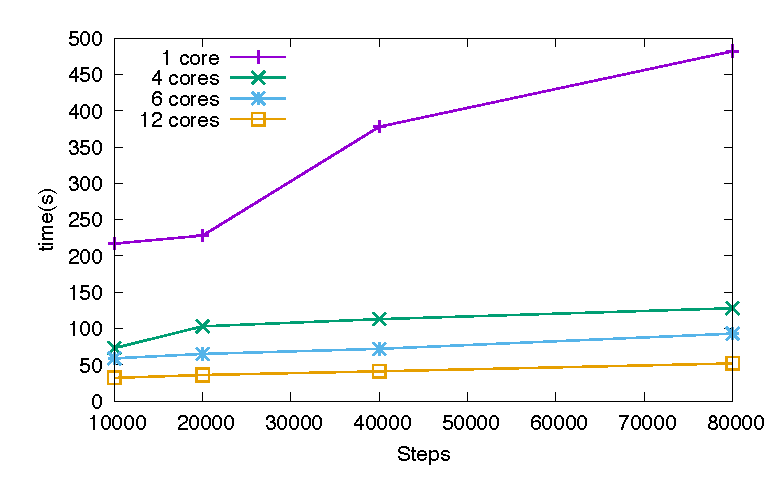
\includegraphics[width=0.75\linewidth]{Chap5/plots/scale.eps}}
\caption[Scalability of KNN2 code on Great Lakes HPC.]{Scalability of KNN2 code for 108,000 atoms on Great Lakes HPC from the University of Michigan with 2x 3.0 GHz Intel Xeon Gold 6154 processors and InfiniBand HDR100 networking, capable of 100 Gb/s throughput.}
\label{Chap:Al/Vac:fig:scale}
\end{figure}
\endgroup


The \ac{KMC} code was written in C++17. \cite{Zhang2020KNN2} Our code has two dependent libraries: 1) We used an open-source C++ module called ``keras2cpp'' to read the Keras model trained in python. \cite{Perevozchikov2019} 2) We also applied another open-source numerical library, called Armadillo \cite{sanderson2016armadillo, sanderson2018user}, to do matrix multiplication for rotating current configurations to symmetry equivalent ones. As we mentioned above, all four symmetry equivalent structures needed to be calculated to evaluate diffusion barriers accurately, and both forward and backward diffusion barriers were required. Therefore, a total of 8 calculations were needed for one event. Therefore it becomes important to speed up calculations. We used \ac{MPI} to parallelize our \ac{KMC} simulations. Two parts are benefited significantly from parallelism implementation: 1) building initial neighbor list of every atom; 2) \ac{KMC} events calculation. Note that once the initial neighbor list is built, one can keep updating the neighbor list on the fly. Besides, diffusion barriers and event rates of 12 possible jumping events of one vacancy were distributed to different cores and collected afterward. We tested the scalability of the code, as shown in Fig. \ref{Chap:Al/Vac:fig:scale}. A (30x30x30) supercell containing 108,000 atoms, was used for this testing. Calculations up to 80,000-steps were tested and benchmarked with the usage of different numbers of nodes. For very limited-steps cases, 10,000-steps for example, more cores showed more advantages, as the initial setup of the neighbor list takes a considerable amount of time. As the simulation goes on, the cost of communication between cores does not affect the scalability significantly.


In order to further speed up \ac{KMC} simulations, a \acf{LRU} Cache, which evict least recently used entry, was implemented based on a hashmap and a  doubly-linked list. Similar idea was practiced by Mason et al.\cite{mason2005fast}. They used Zobrist key to distinguish different binary alloy cluster structures. However, this method ignored detail local environments differences. Instead, we used the 27-digits encoding and store them in an array as the key. The long long int datatype of C++ for a 64-bit machine, can store $2^{64} \sim 1e^{19}$ information. 27-digits encoding scheme with Al, Mg, Zn, and Vac can take up to $4^{27} \sim 1e^{16}$. Therefore, we can simply converting an encoding array to a decimal integer and hash on the decimal integer. The hashmap will hold the keys and the address of the nodes of doubly-linked list . And each node of the doubly-linked list will hold the value of the key, which represents the corresponding diffusion barrier. We will remove elements from the bottom of doubly-linked list and add new elements on top of the bottom of doubly-linked list. And when new entry is accessed, it will be moved to the top again, therefore most recently used entries will always be on the top and least used will be at the bottom of the list. However, by now this implementation only support single core calculations. To make \ac{LRU} Cache available for multiple cores, one way is to sync or share several most recent entries every several thousands of numbers of steps.


Another effort we tried to make \ac{KMC} simulation faster is to boost low-energy barrier event by using \acf{LSKMC} described here in ref. \cite{fichthorn2013local}. The algorithm goes as shown in Algorithm. \ref{algo:lskmc}. Even though the initial and final state of the vacancy is not next to each other in \ac{LSKMC} steps, the corresponding energy change can also be calculated based on a DFS method. Because if the \ac{NN} function to predict the barrier is accurate enough, the energy differences along any path the vacancy takes from the initial site to the final site will be the same. We can do DFS to look for a available path and use the energy changes along the way to get the energy change between two states.

\begin{figure}[!htb]
  \centering
  \begin{minipage}{.75\linewidth}
    \begin{algorithm}[H]
      \caption{\acf{LSKMC} Algorithm from  Ref. \cite{fichthorn2013local}}\label{algo:lskmc}
      \begin{algorithmic}[1]
        \State set $epoch = 0$, $step = 0$, $time = 0$
        \While{$epoch < epoch_{Max}$}
        \State {perform a regular \ac{KMC} step, get time increment $t$.}
        \State {$time$ += $t$}
        \If{$t < t_{critical}$} 
            \State {$step$ += 1} 
        \Else 
            \State {$step = 0$} 
        \EndIf
        \If{$step == step_{critical}$} 
            \State {new superbasin is found.} 
            \State {find transient and absorbing states.}
            \State {compute escape time $t_{escape}$ and probability.}
            \State {decide the exiting states.}
            \State {$time$ += $t_{escape}$}
            \State {$step = 0$} 
        \EndIf
        
        \EndWhile
      \end{algorithmic}
    \end{algorithm}
  \end{minipage}
\end{figure}
\section{Results and Discussion}
\label{Chap:Al/Vac:section:RD}
\subsection{Cluster Searching Algorithm}

In order to better analyzing our results, we have to use a visualization method to characterize clusters. A cluster is a set of connected atoms, each of which is within the range of one or more other atoms from the same cluster. Thus, any two atoms from the same cluster are connected by a continuous path consisting of steps fulfilling the selected neighboring criterion. Adversely, two atoms are not considered in the same cluster if there is no continuous path on the neighbor network leading from one particle to the other. We choose between the distance-based neighbor criterion, in which case two atoms are considered neighbors if they are within the neighbor list of each other. However, in our case, all the atoms are on lattice, so the method described above does not work. It will simply find one huge cluster containing all the atoms. Therefore, we use the method described in Algorithm. \ref{algo:cluster}. We show one typical results in Fig. \ref{Chap:Al/Vac:fig:illu_cluster}. The only top ten clusters are shown. And as you can see, dark red and orange clusters are almost connected. They share one Al atom in common. In that case we treat them as two clusters. Otherwise, if Al atoms are treated like bridges, then most of the atoms in the supercell will be connected as one huge cluster, which is not desired.


\begin{figure}[!htb]
  \centering
  \begin{minipage}{.75\linewidth}
    \begin{algorithm}[H]
      \caption{Cluster Searching Algorithm}\label{algo:cluster}
      \begin{algorithmic}[1]
        \State remove all the solvent atoms (Al for example).
        \State assign an initial cluster id, ($cid = -1$), to all the atoms.
        \State set $count = 0$.
        \For {i in all the solute atoms}
          \If {$cid_i = -1$}
            \State set $cid_i = count$.
            \State \ac{BFS} in the neighbor list of atom i to find other solute atoms and set their $cid = count$.
            \State add their first nearest neighbor solvent atoms (Al for example) back and set their $cid = count$.
            \State $count += 1$.
          \EndIf
        \EndFor
        \State then clusters can be sorted according to any customized methods, by cluster size, element ratios for examples.
      \end{algorithmic}
    \end{algorithm}
  \end{minipage}
\end{figure}


\begingroup
\begin{figure}[!ht]
  \centering
  \subfigure[]{\includegraphics[width=0.49\linewidth]{Chap5/plots/cluster_illu_1.png}}
  \subfigure[]{\includegraphics[width=0.45\linewidth]{Chap5/plots/cluster_illu_2.png}}
\caption[Atomistic pictures of top 10 clusters by size via cluster searching algorithm.]{Atomistic pictures of top 10 clusters by size via cluster searching algorithm. (a) Atomistic pictures of clusters coloring in atom species. Light green, dark green, and red atoms are Al, Mg, and Zn, respectively. (b) Atomistic pictures of clusters coloring in cluster id. The color mapping from dark blue to red is ranked by the cluster size in descending order.}
\label{Chap:Al/Vac:fig:illu_cluster}
\end{figure}
\endgroup


\subsection{Searching for Potential Elements that Can Slow Down Early Stage Nucleation}
\label{Chap:Al/Vac:pseudo}
Similar to the idea of searching ``anchor'' elements in Chap. \ref{Chap:Ag/ZnO:section:anchor}, we will first use \ac{KMC} simulation with some pseudo-atoms (denoted as ``X'') to study their effects on the early stage clustering. In this study, we have Al atoms as solvent atoms, and Mg, Zn atoms as solute atoms. To tune the properties of pseudo atoms, we can change the effects of different elements on vacancy diffusion barriers to the pseudo-atoms, as well as barriers to other elements. We leverage this by adding an offset to the diffusion barrier calculated from \ac{NN} model via Equation. \ref{Chap:Al/Vac:eq:offset} . The amount of the offset is determined by counting first neighbor bonding of X-Al, X-Mg, and X-Zn, via Equation. \ref{Chap:Al/Vac:eq:offset_calculation}:
\begin{subequations}
\begin{align}
{E_a}^{actual} & = {E_a}^{NN} + \textit{offset} \label{Chap:Al/Vac:eq:offset} \\
\textit{offset} & = \sum_{i\in\{Al, Mg, Zn\}} \varepsilon_{i-X} * ( n_{i-X}^{final} - n_{i-X}^{init}) \label{Chap:Al/Vac:eq:offset_calculation}
\end{align}
\end{subequations}
where ${E_a}^{NN}$ is the energy obtained by the neural network prediction of treating element ``X'' as the solvent element Al, the summation is confined to first nearest-neighbors of the vacancy and of the jumping atom, $\varepsilon_{i-X}$ represents the amount of different pairs' effects on the diffusion barrier offset, and $n_{i-X}$ is the number of first nearest neighbor $i-X$ pairs. For example, if $\varepsilon_{Al-X} = 0.01$ that means increasing an Al-X pair will increase the diffusion barrier by a positive 0.01 eV.


The right hand side of Equation. \ref{Chap:Al/Vac:eq:offset} can be divided into two parts. The first part, which is \ac{NN} potential part, can be seen as a more comprehensive bond counting model \cite{soisson1996monte} base on the pair interactions of Al-Al, Al-Mg, Al-Zn, and Mg-Zn, plus cross interactions or higher odered angular contributions. And the second part of the RHS is can be seen as first order bond counting of Al-X, Mg-X, and Zn-X. As a qualitative study, first order pair-wise interaction of the unknown pseudo-atoms should be sufficient. If we rearrange Equation. \ref{Chap:Al/Vac:eq:offset}, we will have:
\begin{subequations}
\begin{align}
{E_a}^{actual} & = \sum_{i, j \in\{Al, Mg, Zn, X\} \& i \neq j} \varepsilon_{i-j} * ( n_{i-j}^{final} - n_{i-j}^{init}) + \textit{H.O.T.(Al, Mg, Zn)} \label{Chap:Al/Vac:eq:rearrange}
\end{align}
\end{subequations}
where $H.O.T$ is the higher order term, such as bond angles. Then the target is to find an element ``X'' that can change the diffusion barrier of Vac-i by roughly the amount of $\varepsilon_{i-X}$, where $i \in \{Al, Mg, Zn\}$.


\begin{table}[!htbp]
\centering
\caption[Sensitivity analysis of different $\varepsilon_{i-X}$.]{Sensitivity analysis of different $\varepsilon_{i-X}$. In the table, the number of different element types are listed.}
\label{Chap:Al/Vac:tab:pseudo1}
\begin{tabular}{cccccccc}
\\
\hline
\hline
setup & $\varepsilon_{Al-X}$  & $\varepsilon_{Mg-X}$  & $\varepsilon_{Zn-X}$ & Al counts & Mg counts & Zn counts & Xe counts\\
\hline
0 &  0.00    &  0.00       &  0.00 & 2106 & 117 &  23 & 126                \\
1 &  0.05    &  0.00       &  0.00 &  867 &  62 &   0 & 108                \\
2 & -0.05    &  0.00       &  0.00 & 4808 & 183 & 109 & 206                \\
3 &  0.05    &  0.05       &  0.00 & 6204 & 274 & 108 & 198                \\
4 &  0.00    & -0.05       &  0.00 & 1927 &  83 &  24 & 117                \\
5 &  0.00    &  0.00       &  0.05 & 8373 & 253 & 150 & 390                \\
6 &  0.00    &  0.00       & -0.05 & 1810 &  87 &  19 & 105                \\
\hline
\hline
\end{tabular}
\end{table}


To setup the simulation for sensitivity tests, we use \ac{LSKMC} method with $step_{critical}$ of 25,000 steps and $E_{critical}$ of 0.3 eV. After around 5 $\sim$ 6 seconds simulation, we can already tell the differences of cluster size obviously. As discussed above, we tuned parameters of $\varepsilon_{i-X}$ for $i \in {Al, Mg, Zn}$. Detailed setup is listed in Table. \ref{Chap:Al/Vac:tab:pseudo1}. And their corresponding final snapshots can be found in Fig. \ref{Chap:Al/Vac:fig:sens_Al}, Fig. \ref{Chap:Al/Vac:fig:sens_Mg}, and Fig. \ref{Chap:Al/Vac:fig:sens_Zn}, respectively. In order to achieve the target of finding a suitable element ``X'', we can use \ac{DFT} with \ac{NEB} to search for elements that can change the diffusion barrier of Vac-i by roughly the amount of $\varepsilon_{i-X}$, where $i \in \{Al, Mg, Zn\}$.


\begingroup
\begin{figure}[!ht]
  \centering
  \subfigure[$\varepsilon_{Al-X} = 0.05$]{\includegraphics[width=0.32\linewidth]{Chap5/plots/cluster_id_jpg/00001.jpg}}
  \subfigure[control]{\includegraphics[width=0.32\linewidth]{Chap5/plots/cluster_id_jpg/00000.jpg}}
  \subfigure[$\varepsilon_{Al-X} = -0.05$]{\includegraphics[width=0.32\linewidth]{Chap5/plots/cluster_id_jpg/00002.jpg}} \\
  \subfigure[$\varepsilon_{Al-X} = 0.05$]{\includegraphics[width=0.32\linewidth]{Chap5/plots/element_jpg/00001.jpg}}
  \subfigure[control]{\includegraphics[width=0.32\linewidth]{Chap5/plots/element_jpg/00000.jpg}}
  \subfigure[$\varepsilon_{Al-X} = -0.05$]{\includegraphics[width=0.32\linewidth]{Chap5/plots/element_jpg/00002.jpg}}
\caption[Atomistic pictures of 108,000 atoms for $\varepsilon_{Al-X}$ sensitivity test.]{Atomistic pictures of 108,000 atoms for $\varepsilon_{Al-X}$ sensitivity test. (a), (d) : $\varepsilon_{Al-X} = 0.05$, which is setup \#1 in Table. \ref{Chap:Al/Vac:tab:pseudo1}. (b), (e) : setup \#0 in Table. \ref{Chap:Al/Vac:tab:pseudo1}. (c), (f) : $\varepsilon_{Al-X} = -0.05$, which is setup \#2 in Table. \ref{Chap:Al/Vac:tab:pseudo1}. (a), (b), and (c) are colored by cluster size. The color mapping from dark blue to red is ranked by the cluster size in descending order. (d), (e), and (f) are colored by atom species. Light green, dark green, and red atoms are Al, Mg, and Zn, respectively.}
\label{Chap:Al/Vac:fig:sens_Al}
\end{figure}
\endgroup

\newpage
\begingroup
\begin{figure}[!ht]
  \centering
  \subfigure[$\varepsilon_{Mg-X} = 0.05$]{\includegraphics[width=0.32\linewidth]{Chap5/plots/cluster_id_jpg/00003.jpg}}
  \subfigure[control]{\includegraphics[width=0.32\linewidth]{Chap5/plots/cluster_id_jpg/00000.jpg}}
  \subfigure[$\varepsilon_{Mg-X} = -0.05$]{\includegraphics[width=0.32\linewidth]{Chap5/plots/cluster_id_jpg/00004.jpg}} \\
  \subfigure[$\varepsilon_{Mg-X} = 0.05$]{\includegraphics[width=0.32\linewidth]{Chap5/plots/element_jpg/00003.jpg}}
  \subfigure[control]{\includegraphics[width=0.32\linewidth]{Chap5/plots/element_jpg/00000.jpg}}
  \subfigure[$\varepsilon_{Mg-X} = -0.05$]{\includegraphics[width=0.32\linewidth]{Chap5/plots/element_jpg/00004.jpg}}
\caption[Atomistic pictures of 108,000 atoms for $\varepsilon_{Mg-X}$ sensitivity test.]{Atomistic pictures of 108,000 atoms for $\varepsilon_{Mg-X}$ sensitivity test. (a), (d) : $\varepsilon_{Mg-X} = 0.05$, which is setup \#3 in Table. \ref{Chap:Al/Vac:tab:pseudo1}. (b), (e) : setup \#0 in Table. \ref{Chap:Al/Vac:tab:pseudo1}. (c), (f) : $\varepsilon_{Mg-X} = -0.05$, which is setup \#4 in Table. \ref{Chap:Al/Vac:tab:pseudo1}. (a), (b), and (c) are colored by cluster size. The color mapping from dark blue to red is ranked by the cluster size in descending order. (d), (e), and (f) are colored by atom species. Light green, dark green, and red atoms are Al, Mg, and Zn, respectively.}
\label{Chap:Al/Vac:fig:sens_Mg}
\end{figure}
\endgroup

\newpage
\begingroup
\begin{figure}[!ht]
  \centering
  \subfigure[$\varepsilon_{Zn-X} = 0.05$]{\includegraphics[width=0.32\linewidth]{Chap5/plots/cluster_id_jpg/00005.jpg}}
  \subfigure[control]{\includegraphics[width=0.32\linewidth]{Chap5/plots/cluster_id_jpg/00000.jpg}}
  \subfigure[$\varepsilon_{Zn-X} = -0.05$]{\includegraphics[width=0.32\linewidth]{Chap5/plots/cluster_id_jpg/00006.jpg}} \\
  \subfigure[$\varepsilon_{Zn-X} = 0.05$]{\includegraphics[width=0.32\linewidth]{Chap5/plots/element_jpg/00005.jpg}}
  \subfigure[control]{\includegraphics[width=0.32\linewidth]{Chap5/plots/element_jpg/00000.jpg}}
  \subfigure[$\varepsilon_{Zn-X} = -0.05$]{\includegraphics[width=0.32\linewidth]{Chap5/plots/element_jpg/00006.jpg}}
\caption[Atomistic pictures of 108,000 atoms for $\varepsilon_{Zn-X}$ sensitivity test.]{Atomistic pictures of 108,000 atoms for $\varepsilon_{Zn-X}$ sensitivity test. (a), (d) : $\varepsilon_{Zn-X} = 0.05$, which is setup \#5 in Table. \ref{Chap:Al/Vac:tab:pseudo1}. (b), (e) : setup \#0 in Table. \ref{Chap:Al/Vac:tab:pseudo1}. (c), (f) : $\varepsilon_{Zn-X} = -0.05$, which is setup \#6 in Table. \ref{Chap:Al/Vac:tab:pseudo1}. (a), (b), and (c) are colored by cluster size. The color mapping from dark blue to red is ranked by the cluster size in descending order. (d), (e), and (f) are colored by atom species. Light green, dark green, and red atoms are Al, Mg, and Zn, respectively.}
\label{Chap:Al/Vac:fig:sens_Zn}
\end{figure}
\endgroup
\section{Conclusion}
\label{Chap:Al/Vac:section:Conc}


In this chapter, Ag-Mg-Zn ternary alloy is used as a model system to simulate the solute clustering kinetics in Al 7000 series alloys. We first demonstrate that the \acf{BEP} relationship, which suggests a simple linear relation between the activation barrier and the reaction energy of one elementary reaction step, fails to provide quantitatively accurate migration barriers of vacancies in these multi-component Al alloys. Then we develop a \ac{NN} model to predict vacancy migration barriers using the training data set of thousands of \ac{DFT} calculated barriers for different alloy configurations. 

A \ac{kMC} method based on this \ac{NN} model is used to study the early transition behavior from a supersaturated solid solution to solute clusters and \acf{GP} zones in Al-Mg-Zn alloys. A local super-basin method  Section \ref{Chap:Al/Vac:sec:LSKMC}, together with \ac{LRU} cache in Section \ref{Chap:Al/Vac:sec:LRU}, is also implemented to accelerate \ac{kMC} simulations. 

We also propose a pseudo-atoms approach to efficiently search the alloying strategy to slow down the solute clustering and the corresponding natural aging effects in Al 7000 series alloys. In this approach, a small number of pseudo-atoms with artificially designed ability to change vacancy migration barriers are added into the Al matrix, and the \ac{kMC} simulations are performed to check their effects to clustering kinetics (so-called ``sensitivity test''). 

We also develop quantitative analysis methods to describe the chemical and structural properties of clusters. Using these quantitative analysis methods, we find that, 1) during the early stage of clustering, Zn-rich clusters appear first, and these clusters become stable very soon, only after 3 seconds; 2) for early-stage clusters, Zn/Mg ratio is converged to 1.2, which is consistent with experimental observations; 3) one possible reason for slightly Zn-rich early-stage clusters is the migration barriers for the vacancy to jump to the adjacent Zn atom is lower than their counterparts for Mg or Al. 

At last, we propose a machine learning strategy based on the structural and chemical information of clusters and precipitates from \ac{kMC} simulations to predict the cluster strengthening and natural aging effects in future studies.